\documentclass{standalone}
\usepackage{tikz}
\usepackage{ctex,siunitx}
\setCJKmainfont{Noto Serif CJK SC}
\usepackage{tkz-euclide}
\usepackage{amsmath}
\usetikzlibrary{patterns, calc,3d}
\usetikzlibrary {decorations.pathmorphing,decorations.pathreplacing,decorations.shapes}
\begin{document}
\small
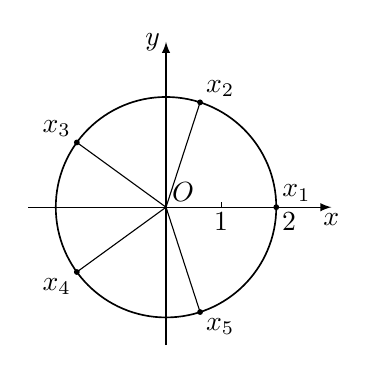
\begin{tikzpicture}[>=latex,scale=0.7,inner sep=2pt]
  \draw[->](-2.5,0)--(3,0)node[below]{$x$};
  \draw[->](0,-2.5)--(0,3)node[left]{$y$};
  \node at (0,0)[above right]{$O$};
  \draw[semithick](0,0)circle(2);
  \draw[very thin](1,0)node[below]{$1$}--++(0,0.1);
  \draw[very thin](2,0)node[below right]{$2$}--++(0,0.1);
  \foreach \x/\y [count=\i from 0] in 
  { 
    1/above right,
    2/above right,
    3/above left,
    4/below left,
    5/below right%
  } 
  {
    \fill(\i*72:2)circle(1.5pt);
    \draw(0,0)--(\i*72:2)node[\y]{$x_\x$};
  }
\end{tikzpicture}
\end{document}